\documentclass[tikz,border=10pt]{standalone}
\usepackage{tikz}
\usepackage{amsmath}

\begin{document}

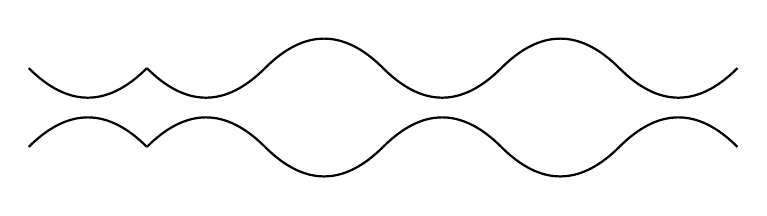
\begin{tikzpicture}[line width=0.8pt]

% First saddle move
\draw (0,0) .. controls (0.5,0.5) and (1,0.5) .. (1.5,0);
\draw (0,1) .. controls (0.5,0.5) and (1,0.5) .. (1.5,1);

% First twist region
\draw (1.5,0) .. controls (2,0.5) and (2.5,0.5) .. (3,0);
\draw (1.5,1) .. controls (2,0.5) and (2.5,0.5) .. (3,1);
\draw (3,0) .. controls (3.5,-0.5) and (4,-0.5) .. (4.5,0);
\draw (3,1) .. controls (3.5,1.5) and (4,1.5) .. (4.5,1);

% Second twist region
\draw (4.5,0) .. controls (5,0.5) and (5.5,0.5) .. (6,0);
\draw (4.5,1) .. controls (5,0.5) and (5.5,0.5) .. (6,1);
\draw (6,0) .. controls (6.5,-0.5) and (7,-0.5) .. (7.5,0);
\draw (6,1) .. controls (6.5,1.5) and (7,1.5) .. (7.5,1);

% Second saddle move
\draw (7.5,0) .. controls (8,0.5) and (8.5,0.5) .. (9,0);
\draw (7.5,1) .. controls (8,0.5) and (8.5,0.5) .. (9,1);

\end{tikzpicture}

\end{document}